\section{Music with Multilayered Temporal Structures}

Based on the research on polyrhythm/cross-rhythm presented above, the following points were taken into consideration when composing the work.

\begin{enumerate}
  \item The definition of polyrhythm: "having beats that are not divisible by integers"
  \item Making this possible through simple rules
  \item Being able to control the sense of groove
\end{enumerate}

These considerations are based on the work titled ''{\bf New York 2997}''\cite{yamato:05}, which the author presented in 2016, where multiple rhythmic cycles wrap around periodically. As can be seen from the explanations so far, polyrhythm/cross-rhythm often exhibits a state where "rhythm fluctuates within a given measure," but I attempted to perform this movement, which is confined within measures, across bar lines. As the author stated in the introduction, if 4/4 meter is dominant in many musical pieces, I thought that by changing the way this 4/4 meter is used, it would be possible to present a sense of rhythm different from existing polyrhythms.

As a prototype for this purpose, I first developed a plugin called ''dc.PolyDelay20'' that runs on Ableton Live. Figure~\ref{fig:figure_25} shows a screenshot of its interface.

\begin{figure}[ht]
\centerline{
	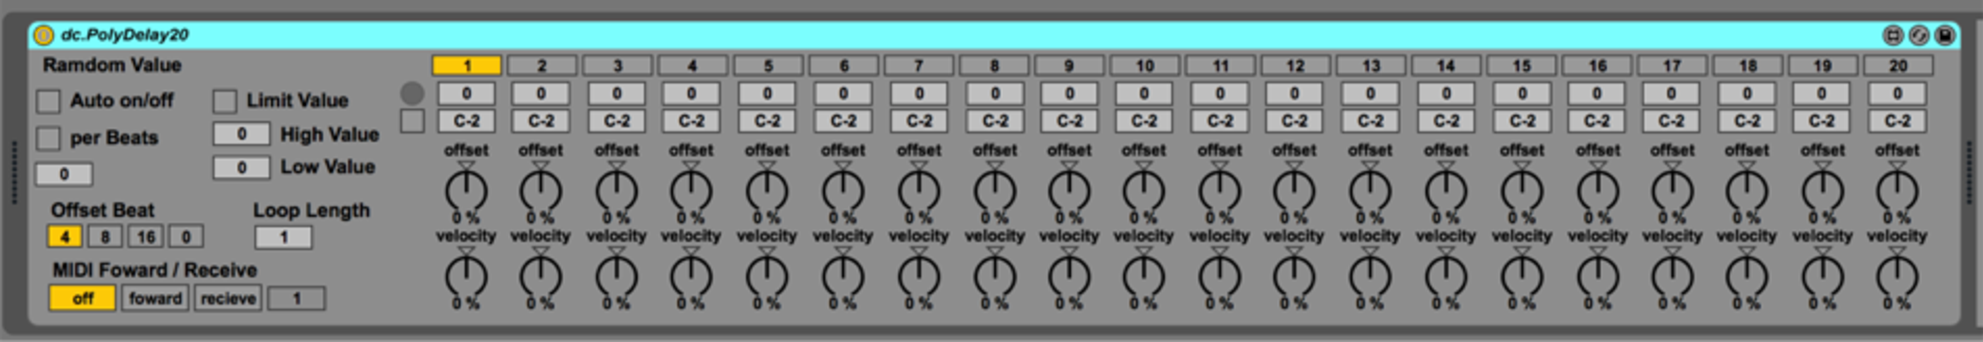
\includegraphics[
 width=\textwidth]{./PDF/figure_25.pdf}
}
\caption{Interface of dc.PolyDelay20}
\label{fig:figure_25}
\end{figure}

This plugin uses MIDI information input as a trigger. By using delay to specify and play up to 20 locations within a specific beat length, it can divide the beat and produce sound at specific timings. Additionally, since pitch information can be varied at that time, it is possible to generate phrases. I repeated prototypes using this plugin. At this time, I created ''{\bf Piano Etude}''\cite{yamato:06} and ''{\bf Percussion Ensemble}''\cite{yamato:07} as compositional prototypes for dividing a certain number of beats into 4 beats. These pieces are created by layering phrases in which lengths from 4 to 13 beats are each divided into 4 beats. The phrases for each piece are shown in Figure~\ref{fig:figure_26} (the same can be downloaded from this URL: \url{https://goo.gl/g3EvW1}) and Figure~\ref{fig:figure_27} (the same can be downloaded from this URL: \url{https://goo.gl/J23Pwi}).

\begin{figure}[ht]
\centerline{
	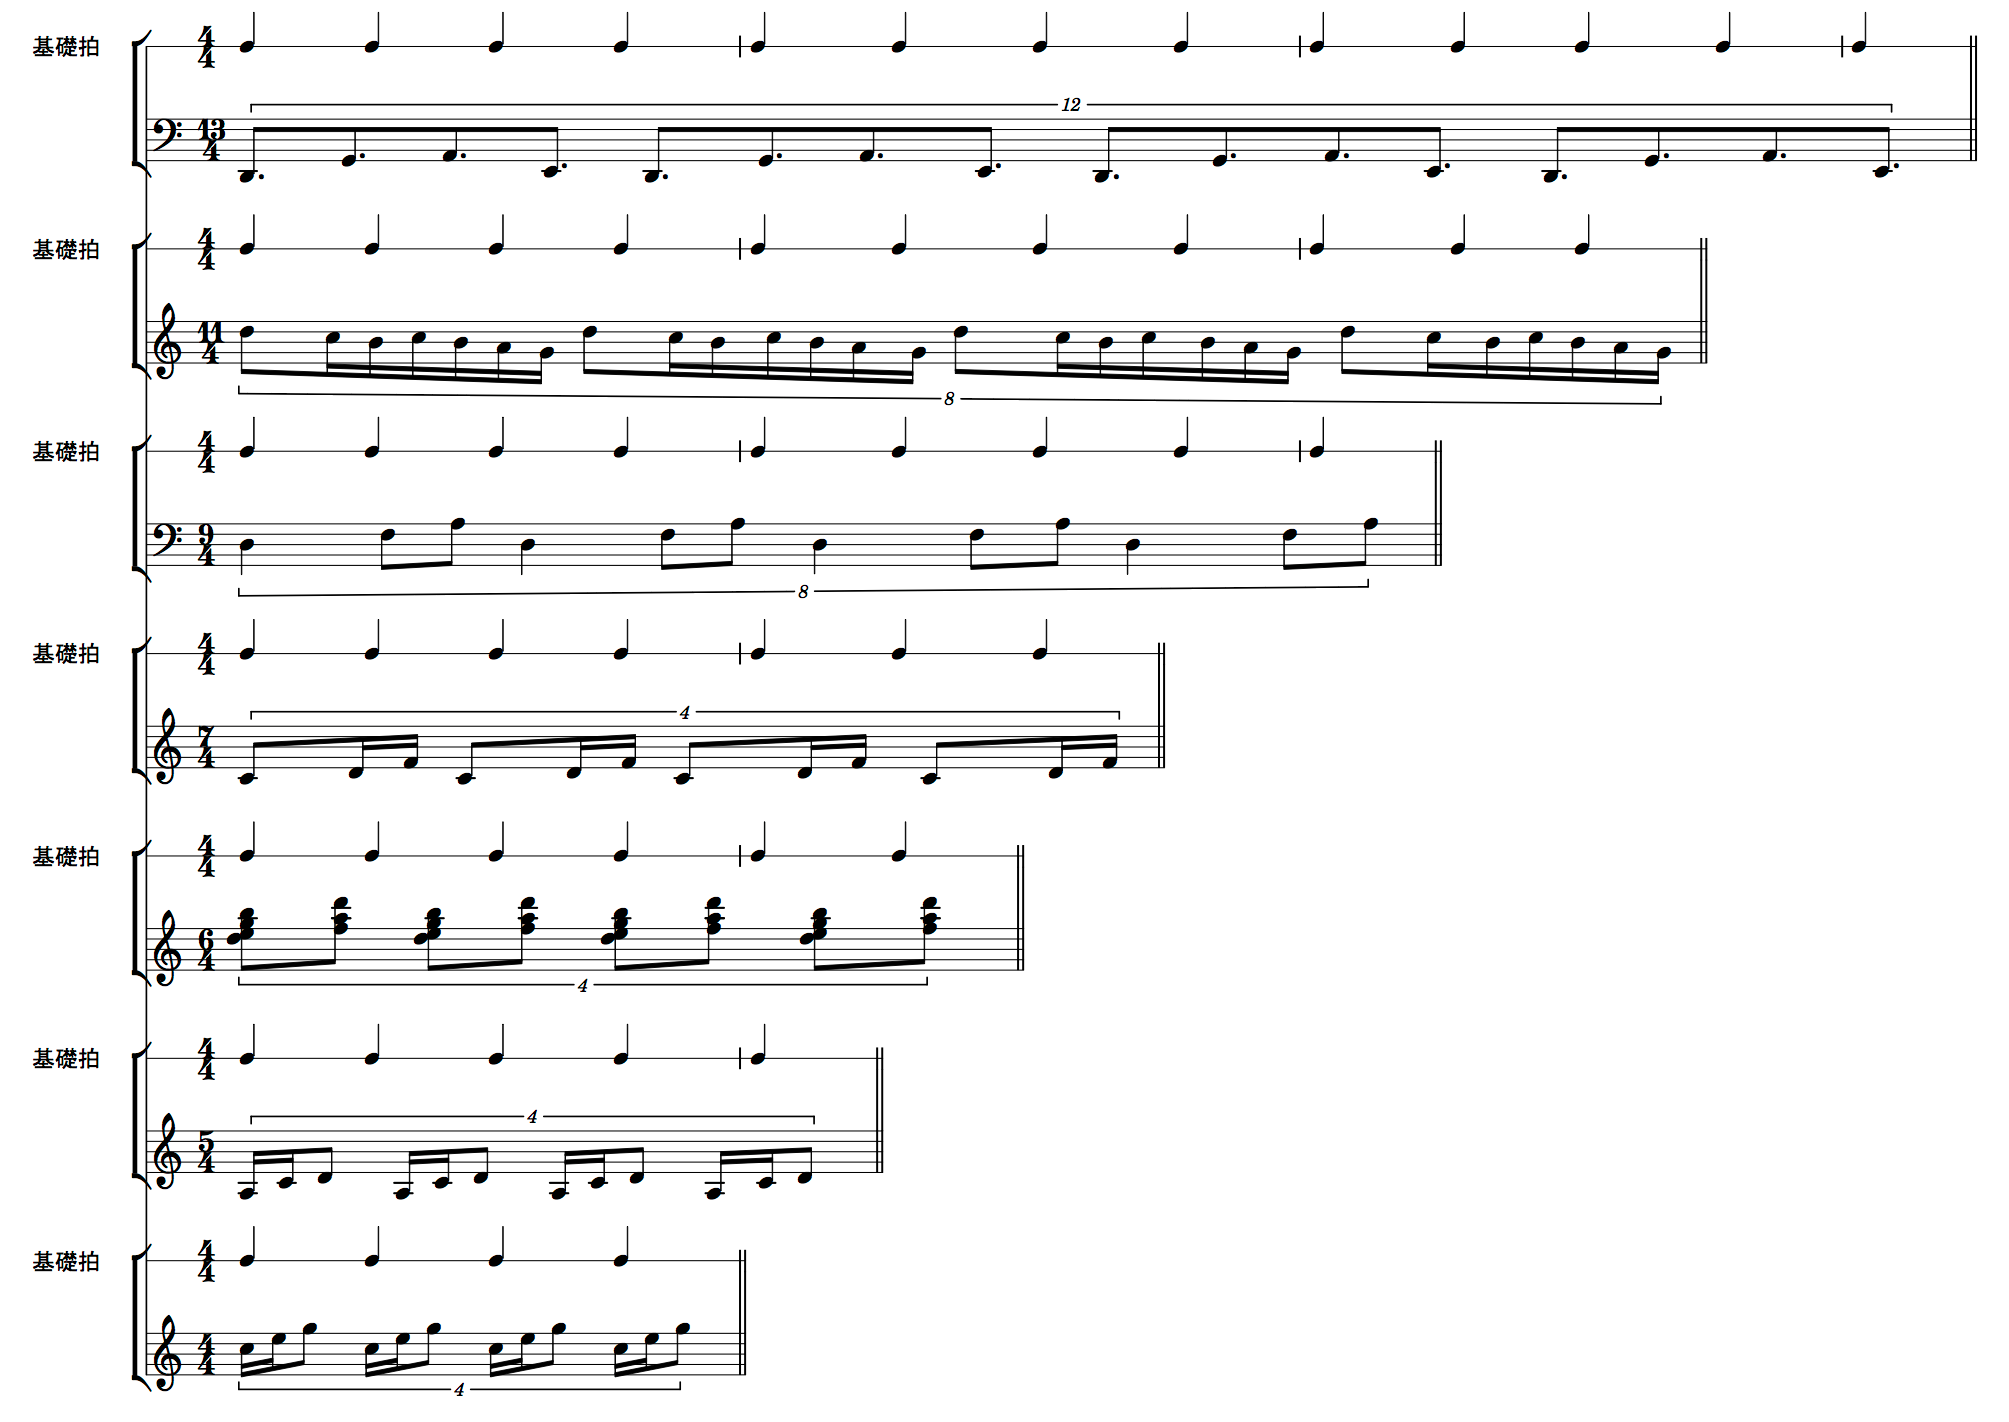
\includegraphics[
 width=\textwidth]{./PDF/figure_26.pdf}
}
\caption{Phrase score of Piano Etude. From top to bottom: 13-beat in 4/4 meter, 11-beat in 4/4 meter, 9-beat in 4/4 meter, 7-beat in 4/4 meter, 6-beat in 4/4 meter, 5-beat in 4/4 meter, 4-beat in 4/4 meter.}
\label{fig:figure_26}
\end{figure}

\begin{figure}[ht]
\centerline{
	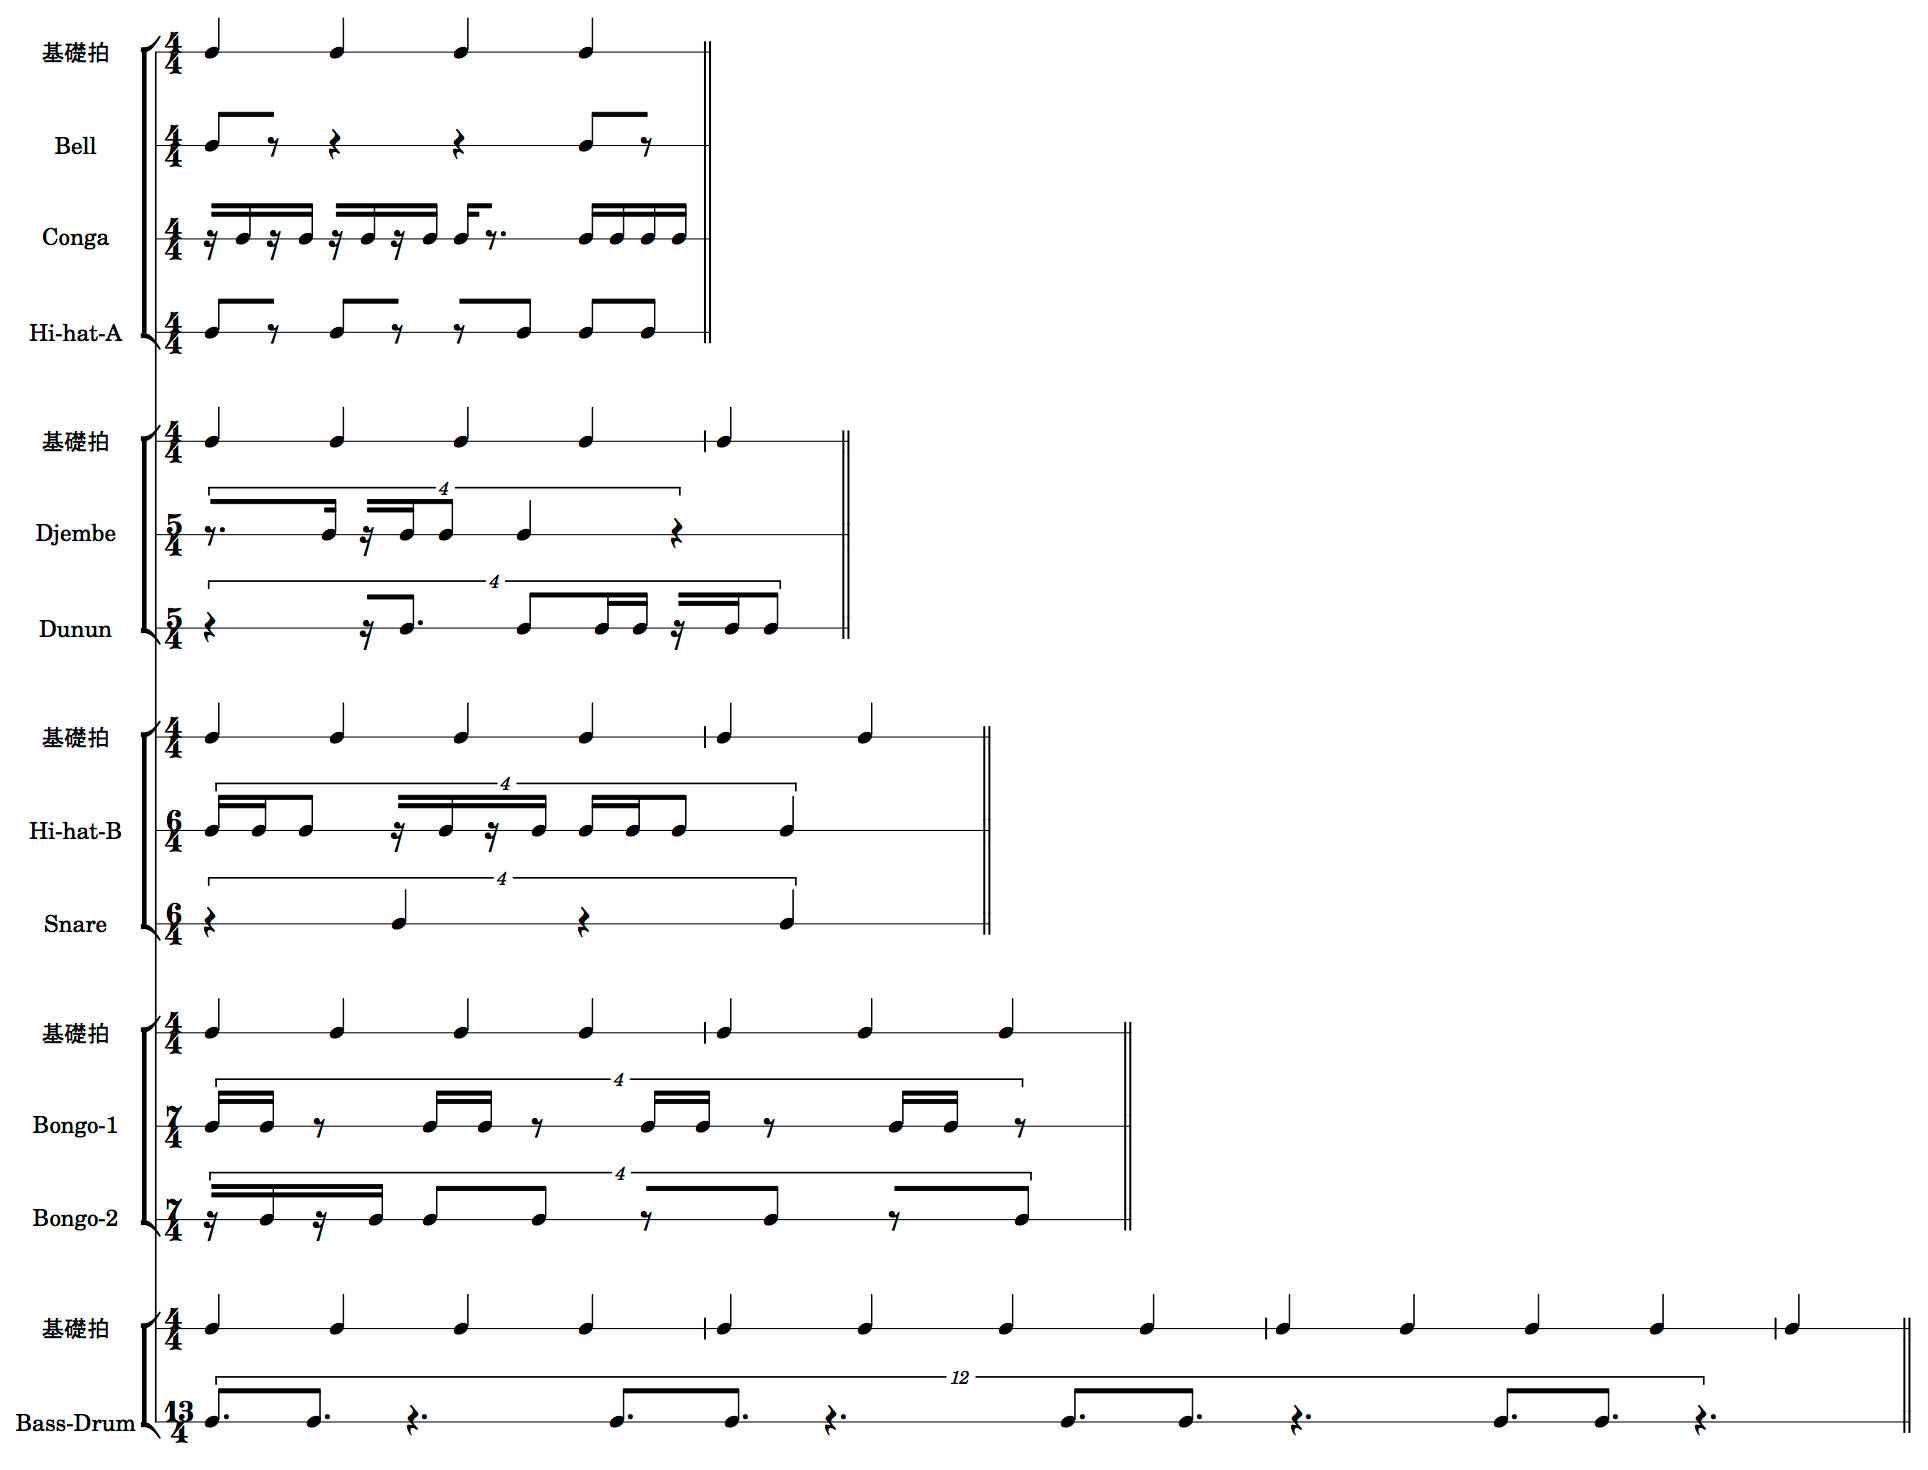
\includegraphics[
 width=\textwidth]{./PDF/figure_27.pdf}
}
\caption{Phrase score of Percussion Ensemble. From top to bottom: 4-beat in 4/4 meter, 5-beat in 4/4 meter, 6-beat in 4/4 meter, 7-beat in 4/4 meter, 13-beat in 4/4 meter.}
\label{fig:figure_27}
\end{figure}

These scores represent each phrase as if written in 4/4 meter, and differ from the actual sounding timings. Figures~\ref{fig:figure_28} (the same can be downloaded from this URL: \url{https://goo.gl/694iHz}) and~\ref{fig:figure_29} (the same can be downloaded from this URL: \url{https://goo.gl/i6J5TM}) show these converted to actual note values.

\begin{figure}[ht]
\centerline{
	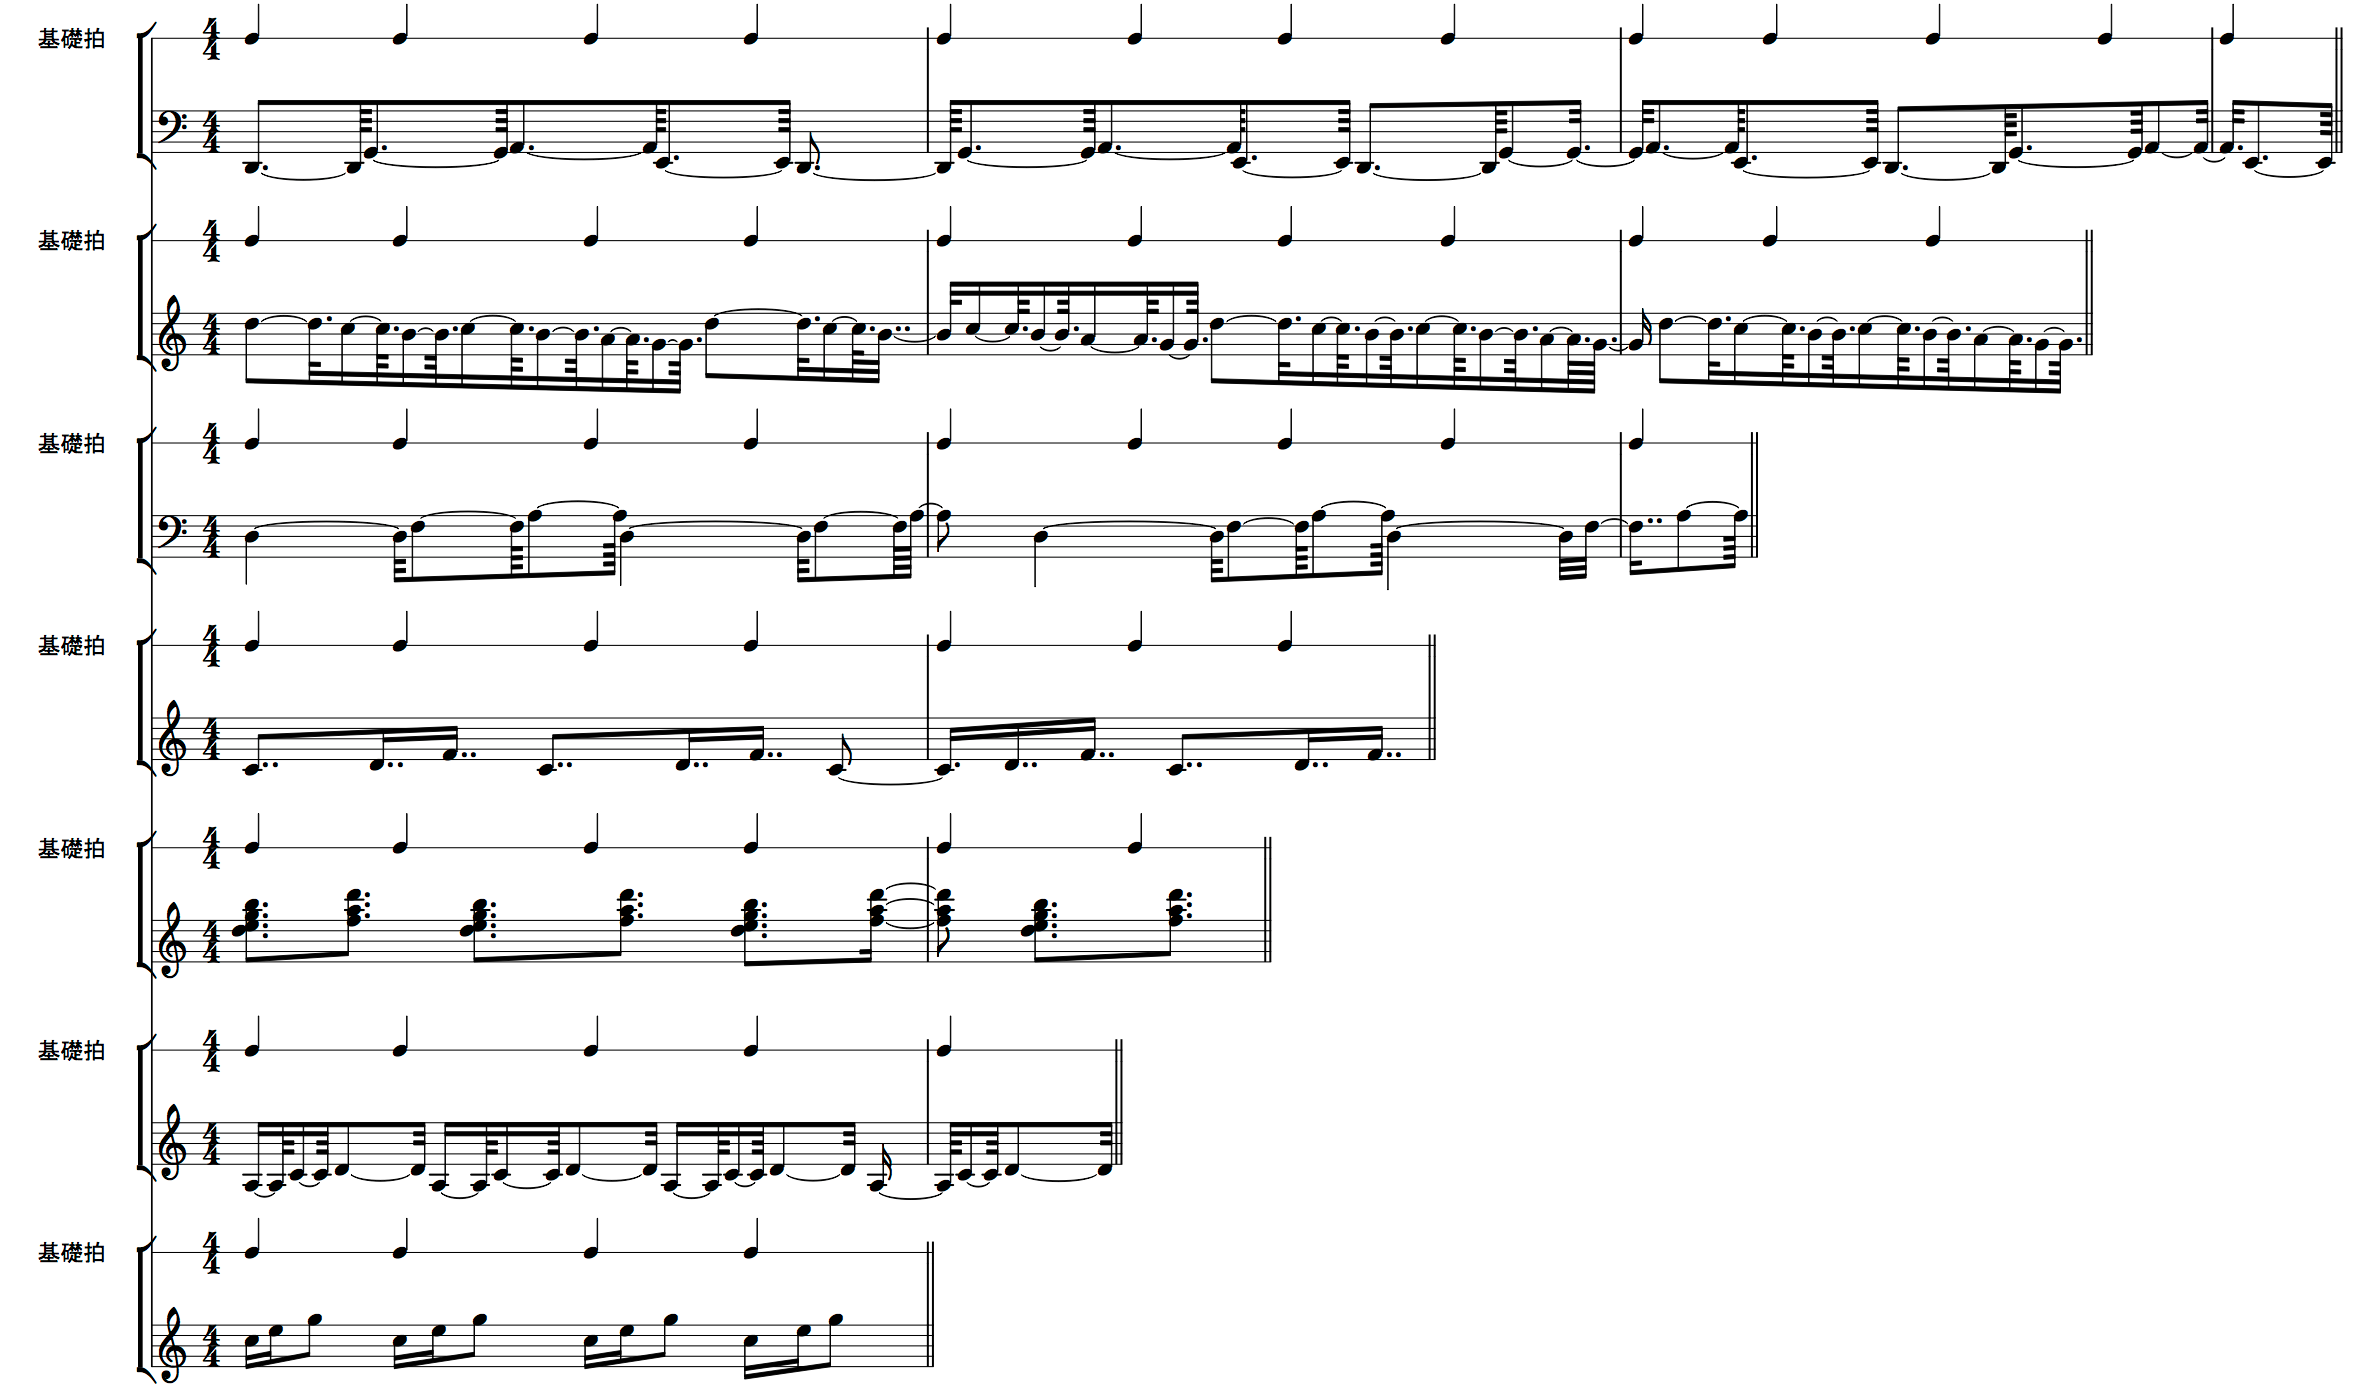
\includegraphics[
 width=\textwidth]{./PDF/figure_28.pdf}
}
\caption{Phrase score of Piano Etude from Figure~\ref{fig:figure_26} converted to actual note values.}
\label{fig:figure_28}
\end{figure}

\begin{figure}[ht]
\centerline{
	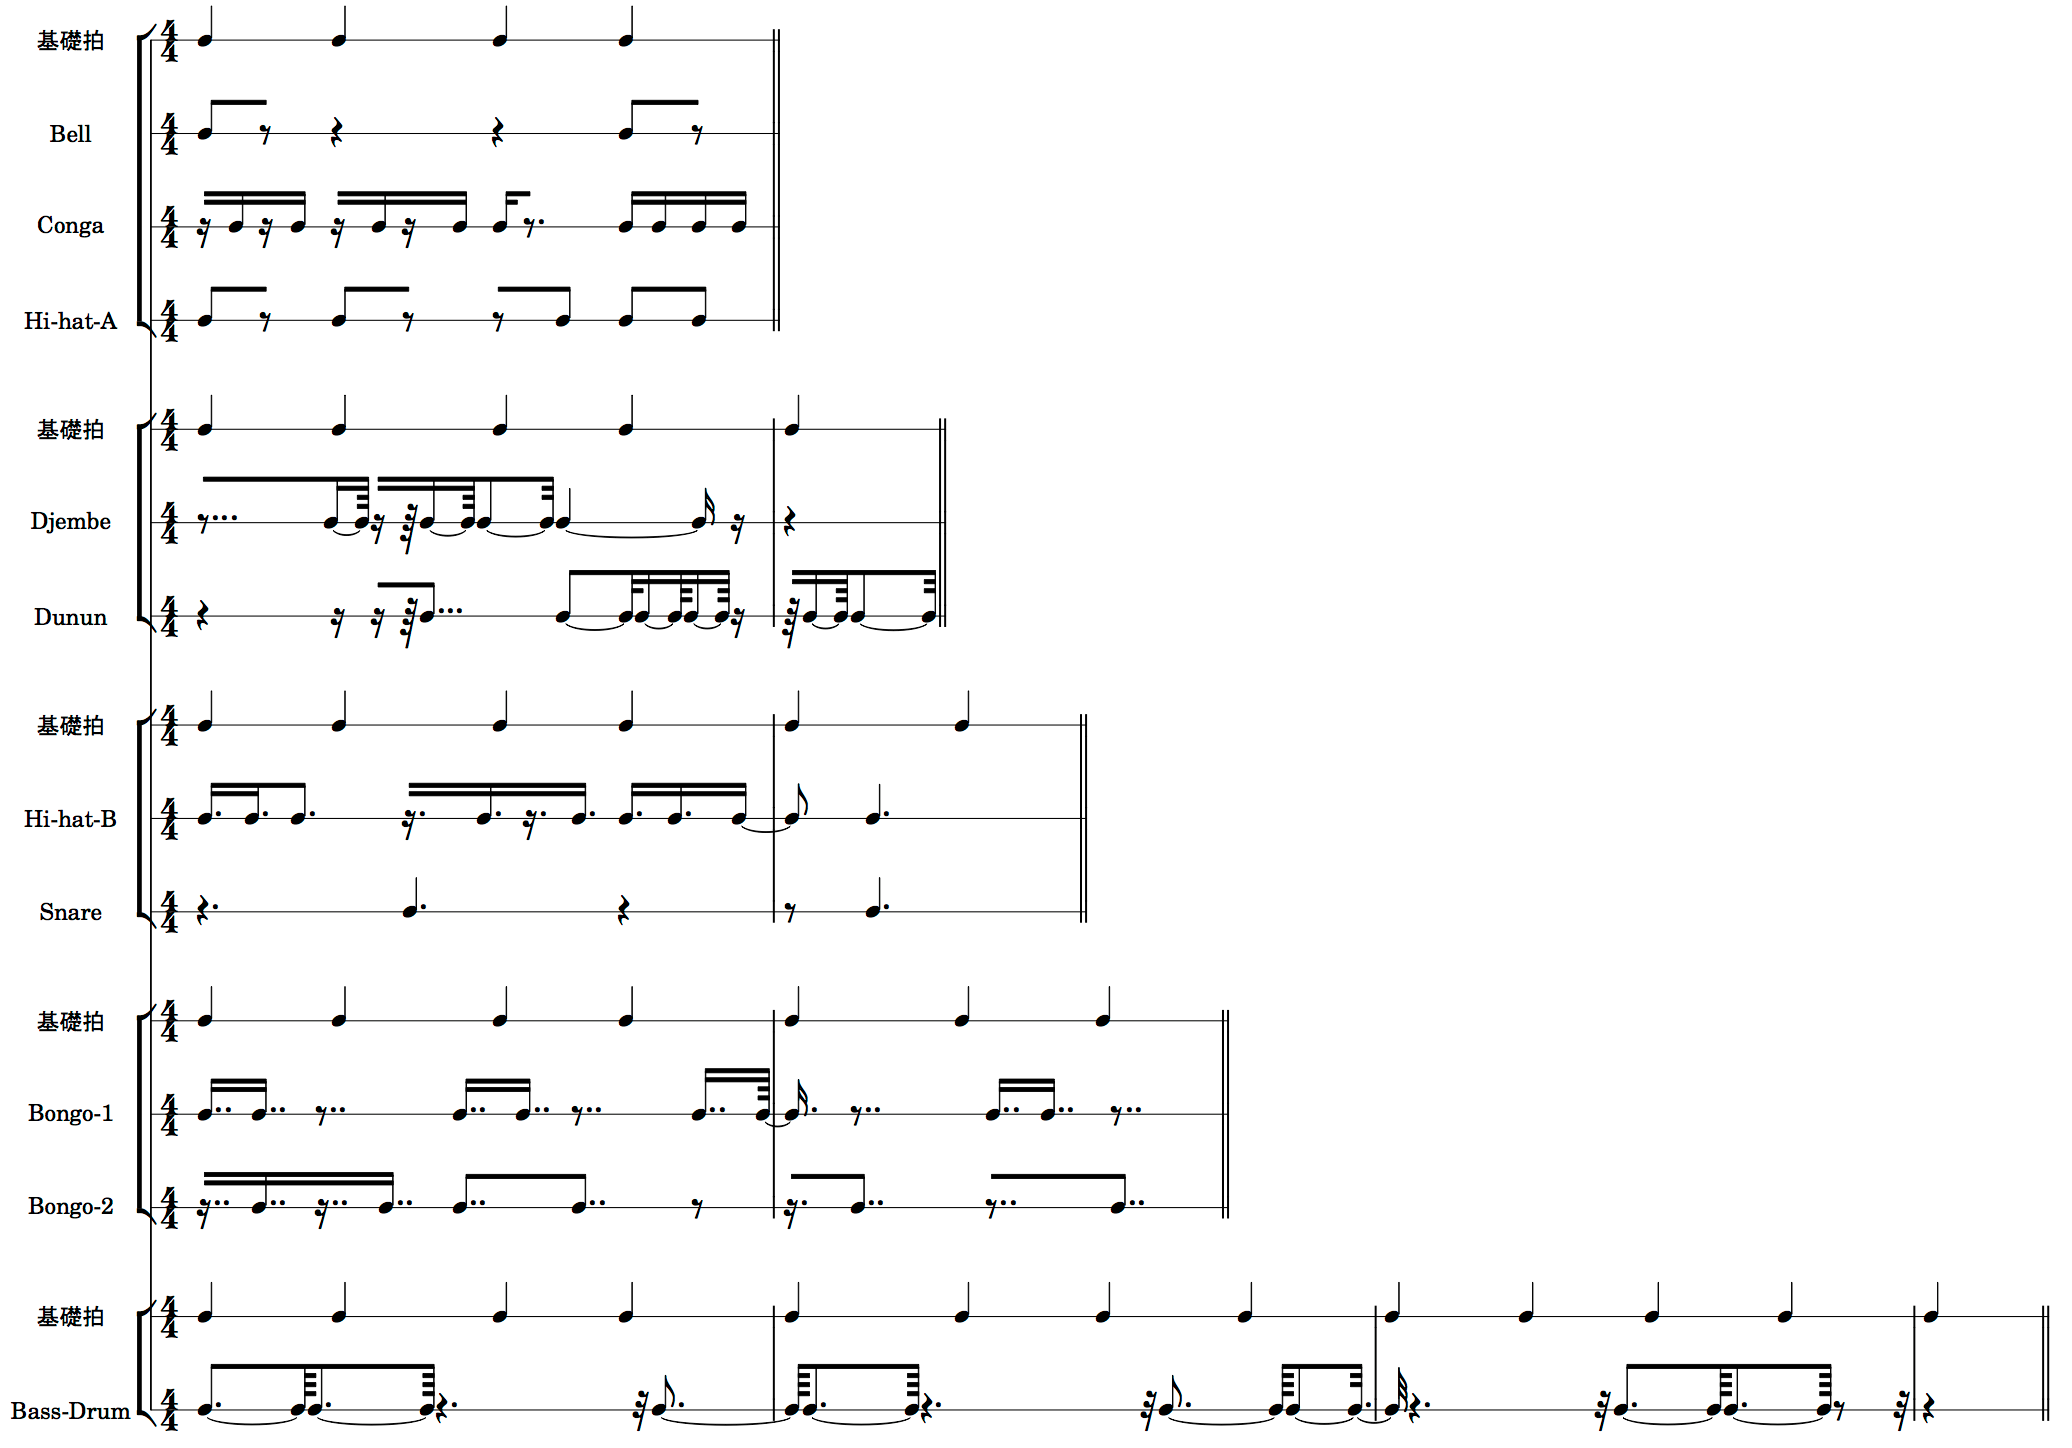
\includegraphics[
 width=\textwidth]{./PDF/figure_29.pdf}
}
\caption{Phrase score of Percussion Ensemble from Figure~\ref{fig:figure_27} converted to actual note values.}
\label{fig:figure_29}
\end{figure}

Through performing division into 4 across bar lines in this way, it became clear that fluctuations and inflections with very fine granularity of note values, which are not seen in conventional musical pieces, can be created through simple rules. It was through these efforts that I conceived what is explained next: "music with multilayered temporal structures."

%改ページや図版を章に収めたい場合は以下のように改ページすると収まる。
\afterpage{\clearpage}
\newpage

\subsection{Definition of "Music with Multilayered Temporal Structures"}

"Music with multilayered temporal structures" is largely defined by the following two elements:

\begin{enumerate}
  \item Lines (melodies, rhythms, instrumental parts) of different tempos flow simultaneously
  \item The lines of different tempos in item 1 "periodically align at the first beat of a certain measure"
\end{enumerate}

To put it simply, it is "music made up of multiple layers of $ n $-beat in 4/4 meter at different BPMs," but unlike so-called random multi-BPM or free tempo, the characteristic feature is that beats align at a certain cycle.

\begin{figure}[ht]
\centerline{
	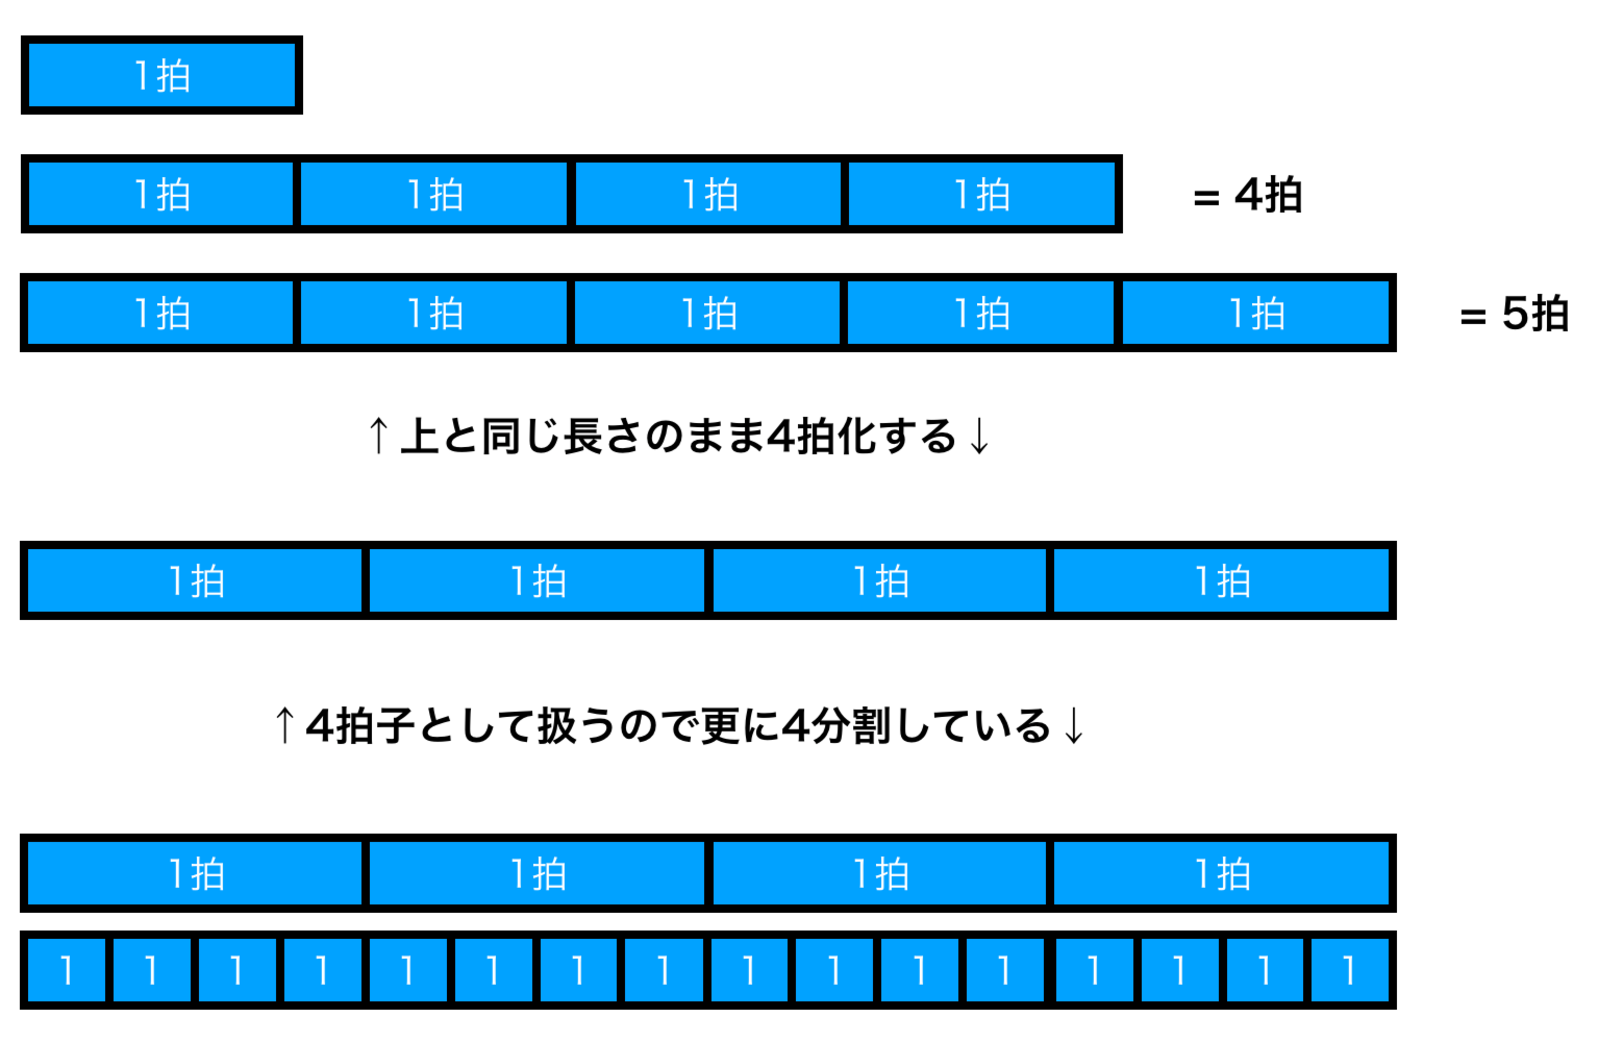
\includegraphics[
 width=\textwidth]{./PDF/figure_01.pdf}
}
\caption{Diagram showing the process of creating 5-beat in 4/4 meter from the common beat of 4-beat in 4/4 meter. By arranging five 1-beat units of 4-beat in 4/4 meter, one can create 5-beat in 5/4 meter. By converting this length as-is into quadruplets, it becomes 5-beat in 4/4 meter. Also, by dividing 1 beat into 4 as the basic grid of 4/4 meter, one can create the 16th note grid for 5-beat in 4/4 meter.}
\label{fig:figure_01}
\end{figure}

Figure~\ref{fig:figure_01} shows the concept of 5-beat in 4/4 meter in the case of multiple layers of 4-beat in 4/4 meter and 5-beat in 4/4 meter. First, based on the length of one beat in 4-beat in 4/4 meter (that is, normal 4/4 meter), take the length of 5 beats. Convert this length as-is into 4 beats (in other words, it becomes synonymous with 5-beat quadruplets). At that time, by treating both as 4/4 meter without sharing bar lines, 4/4 meters with different tempos are layered. Furthermore, since these 4-beat in 4/4 meters originally had lengths of 4 and 5 beats respectively and share the length of one beat, the beat attack points align at the downbeat of the next measure (21st beat) following the 4th beat of the 5th measure corresponding to the 20th beat on the 4-beat in 4/4 meter side, and at the downbeat of the next measure (17th beat) corresponding to the 16th beat on the 5-beat in 4/4 meter side. Although this is a simple least common multiple, the $ n $-beat in 4/4 meters of both sides do not align at the beginning of measures in between, and they cycle while causing a displacement of at least 16th notes.

This simple method of layering $ n $-beat in 4/4 meter is the basic concept of "music with multilayered temporal structures."

\subsection{Notation in "Music with Multilayered Temporal Structures"}
Regarding notation in "music with multilayered temporal structures," as can be seen from the previous prototype examples, conventional notation becomes difficult to read. Therefore, in order to clearly show the composer's subjective view while ensuring readability, I use notation called "variable meter notation" and "fixed meter notation." Below, I will explain each based on the pieces included in the work ''Music for multilayered temporal structures''. Figure~\ref{fig:figure_02} below corresponds to the Drum part of the piece ''Etude \#1'' included in the same work.

\begin{figure*}[htb]
\centerline{
	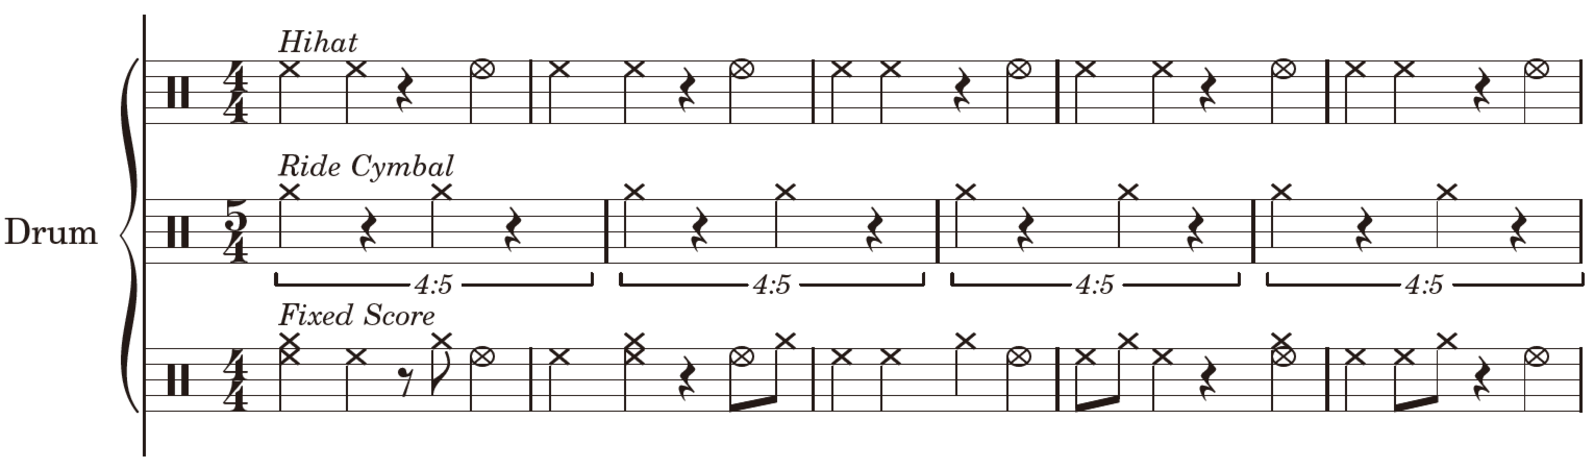
\includegraphics[
 width=\textwidth]{./PDF/figure_02.pdf}
}
\caption{Drum part of Etude \#1 INTRO section}
\label{fig:figure_02}
\end{figure*}

In the score example of Figure~\ref{fig:figure_02}, the top two staves show the "variable meter notation" score of the multiple layers of 4-beat in 4/4 meter and 5-beat in 4/4 meter. The characteristic of variable meter notation is that, in the case of this score, since it becomes multiple layers of $ n $-beat in 4/4 meter, bar lines are not shared between 4-beat in 4/4 meter and 5-beat in 4/4 meter, and the phrases wrap around. Also, although the 5-beat in 4/4 meter side is equivalent to so-called "5-beat quadruplets," with ordinary tuplet note values it is not possible to show the concept of $ n $-beat in 4/4 meter that "bar lines wrap around and the length of the fundamental beat is different," so tuplet symbols are indicated as "4:5" and aligned in notation with the note values of each 4/4 meter.

In contrast, the part indicated as "Fixed Score" in the third staff of the same score example corresponds to "fixed meter notation." This is the "variable meter notation" of the top two staves compiled into a form with aligned bar lines (here, 4-beat in 4/4 meter), and corresponds to what is generally called conventional score format.

Also, in ''Etude \#3'' included in the same work, it is necessary to use notation as shown in Figure~\ref{fig:figure_03}.

\begin{figure*}[htb]
\centerline{
	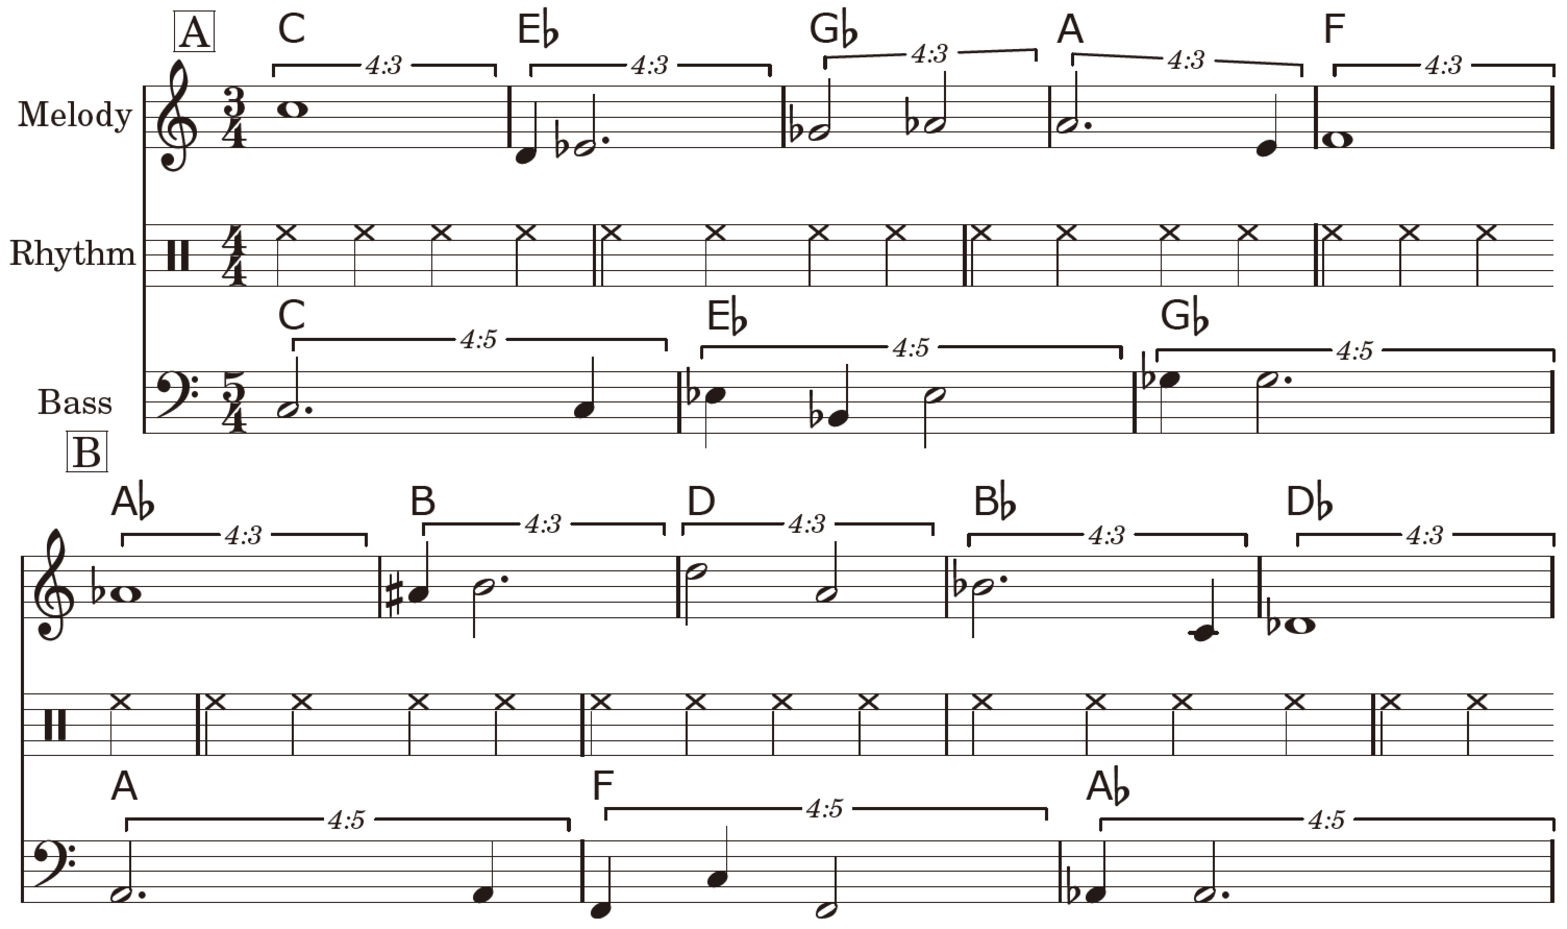
\includegraphics[
 width=\textwidth]{./PDF/figure_03.pdf}
}
\caption{Etude \#3 [A][B] section}
\label{fig:figure_03}
\end{figure*}

''Etude \#3'' is composed in three layers: 3-beat in 4/4 meter, 4-beat in 4/4 meter, and 5-beat in 4/4 meter. This is an example of its "variable meter notation," but 3-beat in 4/4 meter (first staff of the score example) and 5-beat in 4/4 meter (third staff of the score example) align at the end of measures after 5 measures and 3 measures respectively, similar to the previous ''Etude \#1''. In contrast, 4-beat in 4/4 meter (second staff of the score example) needs to wrap to the next line in the middle of a bar line.

In this way, notation that would normally be treated as a taboo in reading conventional score formats becomes necessary, which is one characteristic of music with "multilayered temporal structures," and this raises awareness of problems with the score as a "system that guarantees performability" and "the environment itself related to music production," while simultaneously connecting to "new musical experiential characteristics with diversity" born from rhythm.

\subsection{Rhythm in "Music with Multilayered Temporal Structures"}

Next, I will explain rhythm in "music with multilayered temporal structures."

First, as mentioned earlier, the basic cycle of rhythm in "music with multilayered temporal structures" is the multiple layers of "$ n $-beat," meaning in the case of layers of 4-beat and 5-beat units like "Etude \#1" and "Etude \#2," it can be considered a cycle with 20 as the least common multiple. Just as the 3:4 rhythm of Africa mentioned earlier can be shown as 12/8 meter divided into 3+3+3+3 and 4+4+4 respectively, in the case of a 4:5 rhythm, if converted to one measure, it becomes 20/16 meter, which takes the form of vertical hemiola with 4+4+4+4+4 and 5+5+5+5 respectively, and this has fundamentally the same structure as basic African polyrhythm (cross-rhythm in the definition of this paper). Even with 3:4:5 in "Etude \#3," although the least common multiple is 60 and the cycle at which phrase wraparound aligns becomes larger compared to 4:5, it remains vertical hemiola as is. In order to generate polyrhythmic fluctuation from this vertical hemiola, each $ n $-beat was converted into 4/4 meter.

The specific method for calculating beat attack points is as follows. The beat $ N $ at which "multiple layers of $ n $-beat in 4/4 meter with polyrhythmic fluctuation align at the downbeat point of the measure" is the beat obtained by adding 1 to the least common multiple $ LCM $ of each $ n $-beat. Next, by dividing the least common multiple $ LCM $ by $ n $-beat, the number of measures $ bars $ can be calculated. Furthermore, by multiplying the number of measures $ bars $ by 4, the number of quarter notes $ beats $ until each $ n $-beat in 4/4 meter aligns at the downbeat can be determined (multiplying by 8 gives the number of eighth notes). The above can be shown by the following simple formula:\\

\begin{math}
beats = LCM \div n \times 4
\end{math}\\

By dividing $ LCM $ by the obtained $ beats $, the length of one beat $ length $ for each $ n $-beat in 4/4 meter can be calculated.\\

\begin{math}
length = LCM \div beats
\end{math}\\

By multiplying this by values from 1 to the maximum value $ m $ of $ beats $, the position of each beat $ p $ can be calculated from $ LCM $.\\

\begin{math}
(p_1,p_2\dots,p_m) = length \times (beats_1,beats_2\dots,beats_m)
\end{math}\\

By relativizing these values and comparing each $ n $-beat in 4/4 meter, the common beats of each $ n $-beat in 4/4 meter can be determined. For actual comparison, I initially used hand calculations on graph paper, and later used a program implemented on openFrameworks. The common beat attack points obtained from this comparison are used as rhythmic motifs in the composition. The programs used, ''4by5''\cite{yamato:02} and ''3by4by5''\cite{yamato:03}, are published in the author's GitHub repository.

Also, as mentioned earlier, the concept of multiple layers of $ n $-beat in 4/4 meter can be called multiple layers of "4/4 meter at different BPMs." In this case, each $ BPM $ can be calculated by the following formula when the basic BPM is $ BaseBPM $:\\

\begin{math}
BPM = BaseBPM \div ( n \div 4 )
\end{math}\\

For example, in the case of ''Etude \#1'', the speed of the basic 4/4 meter is specified as 115 BPM. When applied to the above formula, while 4-beat in 4/4 meter is 115 BPM, 5-beat in 4/4 meter is $ 115 \div ( 5 \div 4 ) = 92 $, or 92 BPM, and it can be seen that it is multiple layers of BPMs in integer ratio 5:4. However, when calculating the BPM of 3-beat in 4/4 meter against this 115 BPM 4-beat in 4/4 meter, it becomes $ 115 \div ( 3 \div 4 ) = 153.333\dots $, and the multiple layers of BPMs can no longer be captured in integer ratios. If the basic BPM is something like 120, all integer ratios can be created, but depending on the basic BPM, it does not become an integer ratio. From this as well, it can be understood that this method can create rhythmic beat attack points with polyrhythmic characteristics that cannot be processed by simple BPM conversion when using programs, etc., using simple rules.

Next, as concrete examples of rhythmic beat attack points, Figure~\ref{fig:figure_04} shows the rhythmic motifs used in "4-beat in 4/4 meter" and "5-beat in 4/4 meter" of ''Etude \#1'' and ''Etude \#2''. In ''Etude \#1'' and ''Etude \#2'', the rhythmic motifs use common beats compared in eighth notes. The green indicates the common beat attack points, but if only those beats were used, the groove of the 4-beat in 4/4 meter side would be lost, so the downbeats of 4-beat in 4/4 meter are also added to the rhythmic motif to express the multiple layers of 4-beat in 4/4 meter and 5-beat in 4/4 meter. Also, Figure~\ref{fig:figure_05} shows this beat attack point notated in "variable meter notation."

\begin{figure*}[htb]
\centerline{
	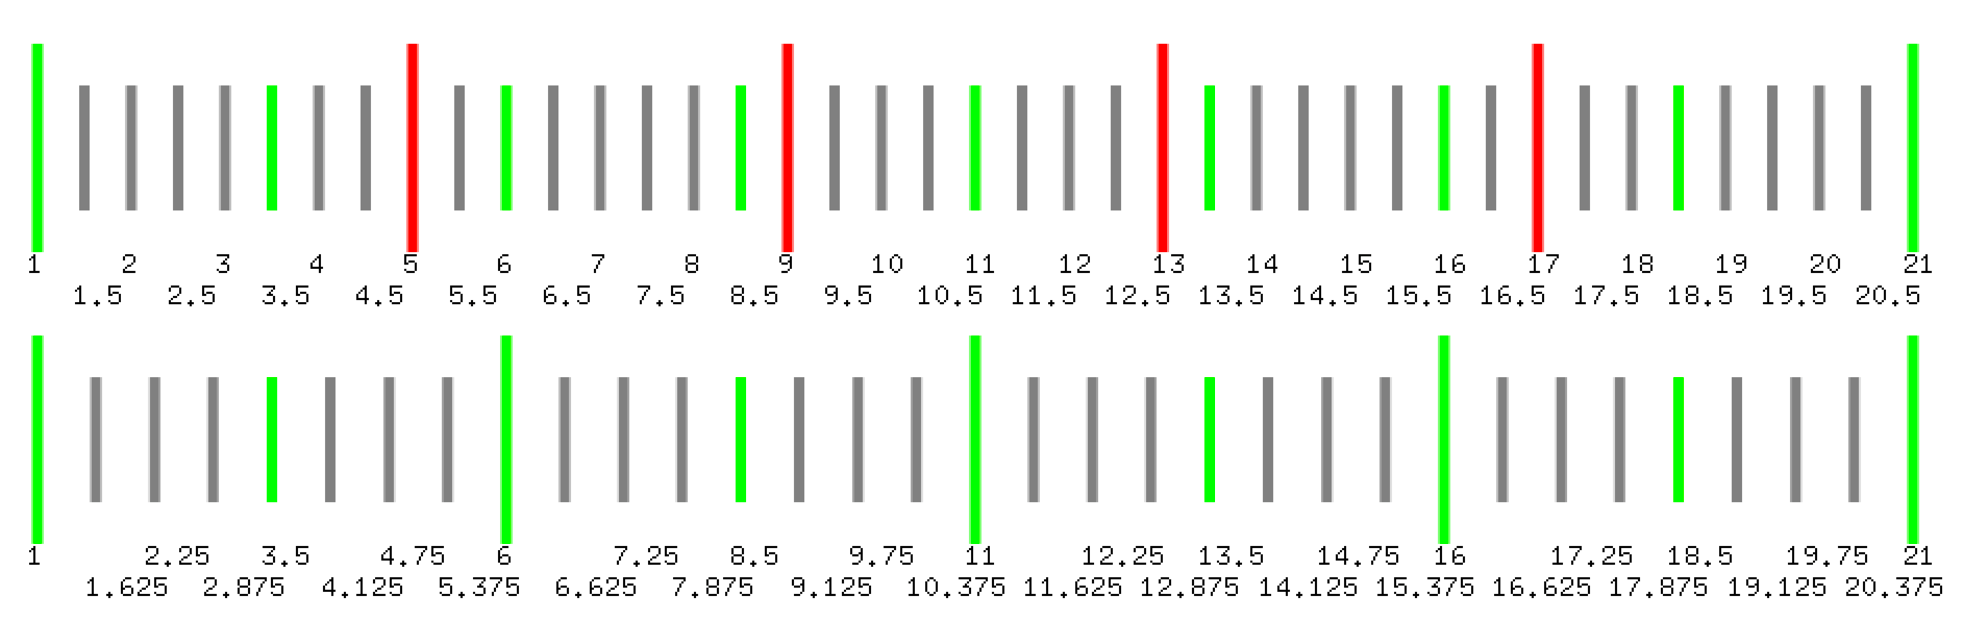
\includegraphics[
 width=\textwidth]{./PDF/figure_04.pdf}
}
\caption{Rhythmic motif diagram of ''Etude \#1'' and ''Etude \#2''. The top of the figure shows the eighth note beat attack points of 4-beat in 4/4 meter. The bottom shows the eighth note beat attack points of 5-beat in 4/4 meter. The green lines indicate the common beat attack points of each. The red lines indicate beat attack points arbitrarily added as rhythmic motifs. The numbers written below the lines numerically indicate the position of each beat attack point.}
\label{fig:figure_04}
\end{figure*}

\begin{figure*}[htb]
\centerline{
	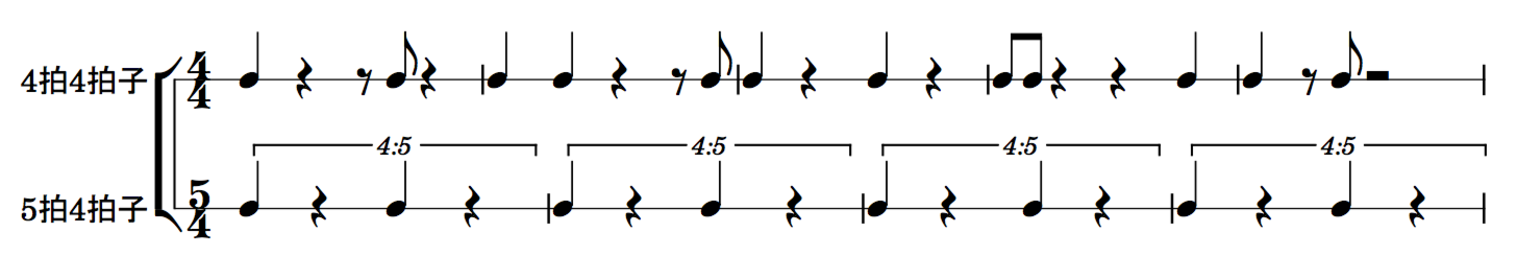
\includegraphics[
 width=\textwidth]{./PDF/figure_05.pdf}
}
\caption{Example showing Figure~\ref{fig:figure_04} in variable meter notation}
\label{fig:figure_05}
\end{figure*}

Next, Figure~\ref{fig:figure_06} shows the rhythmic motif diagram used in the three-layer piece "3-beat in 4/4 meter," "4-beat in 4/4 meter," and "5-beat in 4/4 meter" in ''Etude \#3''. In the actual piece, "4-beat in 4/4 meter" intentionally does not use common beat attack points for compositional purposes.

\begin{figure*}[htb]
\centerline{
	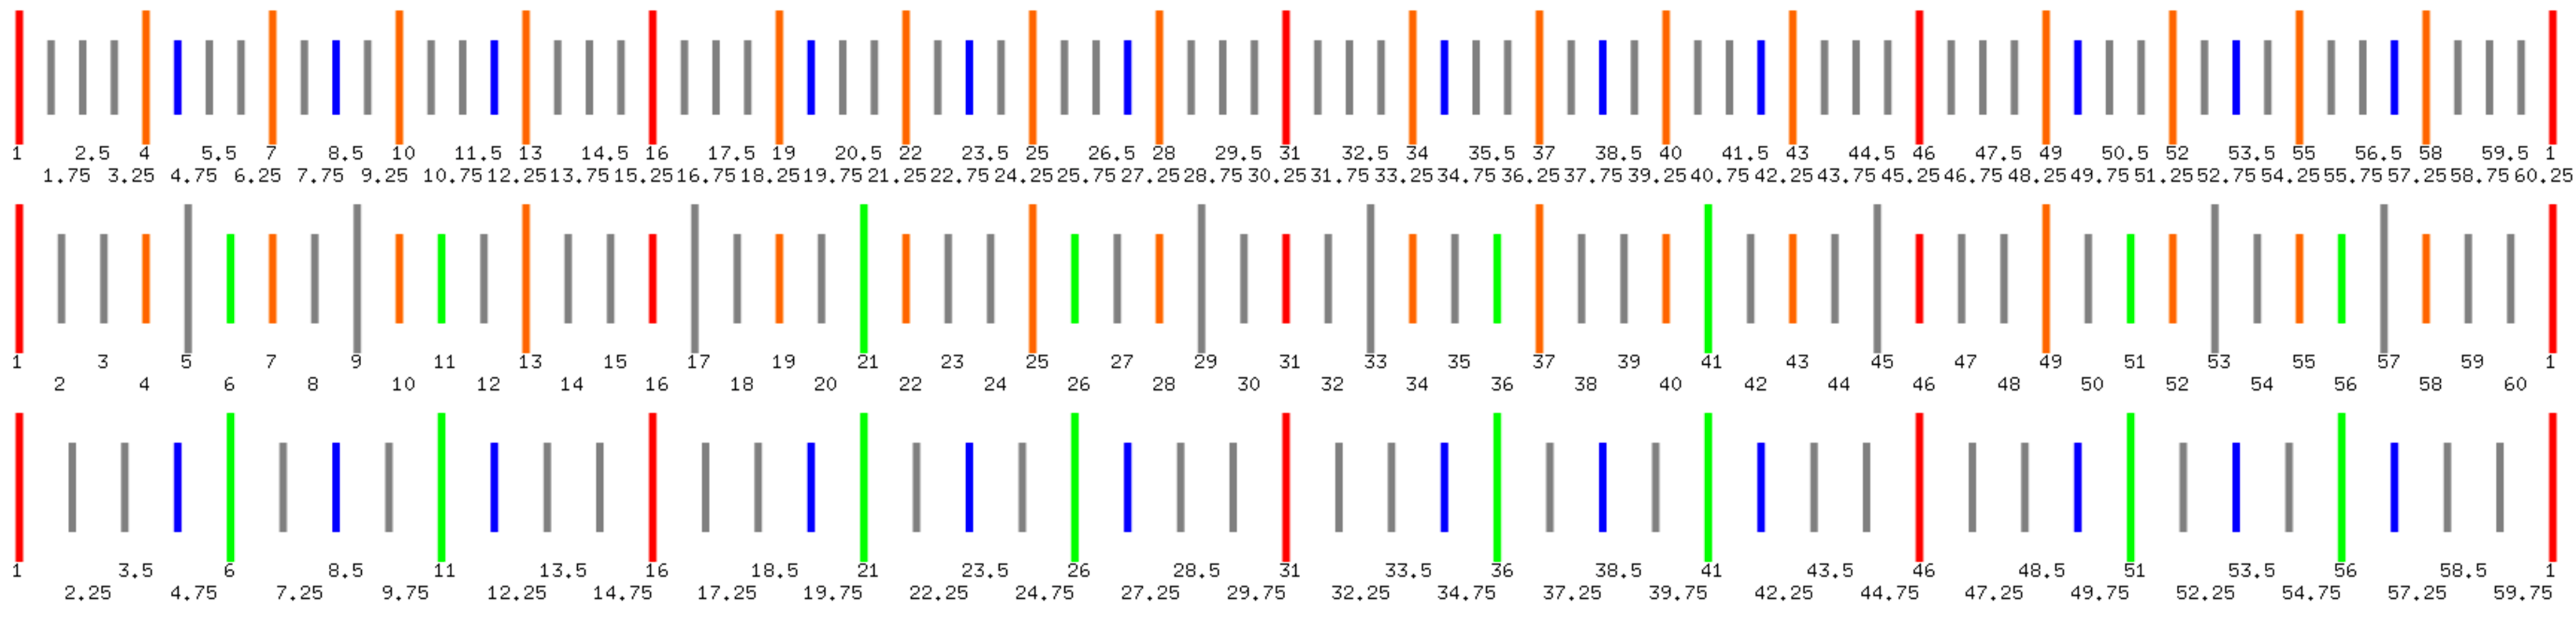
\includegraphics[
 width=\textwidth]{./PDF/figure_06.pdf}
}
\caption{Rhythmic motif diagram of ''Etude \#3''. From top to bottom, showing the beat attack points in quarter notes for 3-beat in 4/4 meter, 4-beat in 4/4 meter, and 5-beat in 4/4 meter. Red indicates beat attack points common to all three meters, orange indicates beat attack points common to 3-beat in 4/4 meter and 4-beat in 4/4 meter, green indicates beat attack points common to 4-beat in 4/4 meter and 5-beat in 4/4 meter, and blue indicates beat attack points common to 3-beat in 4/4 meter and 5-beat in 4/4 meter. Although not visible in the figure display, the numerically expressed position of each beat attack point is shown below each beat attack point, as in Figure~\ref{fig:figure_04}.}
\label{fig:figure_06}
\end{figure*}

This method of using common beats as rhythmic motifs creates relationships between each $ n $-beat in 4/4 meter, making it possible to achieve structural understanding when performing, and each performer can generate the pulse of their respective rhythm themselves. Figure~\ref{fig:figure_07} shows an explanation of "how to take beat attack points" for achieving "structural understanding of rhythm in variable meter notation" explained in the work ''Music for multilayered temporal structures''.

\begin{figure*}[htb]
\centerline{
	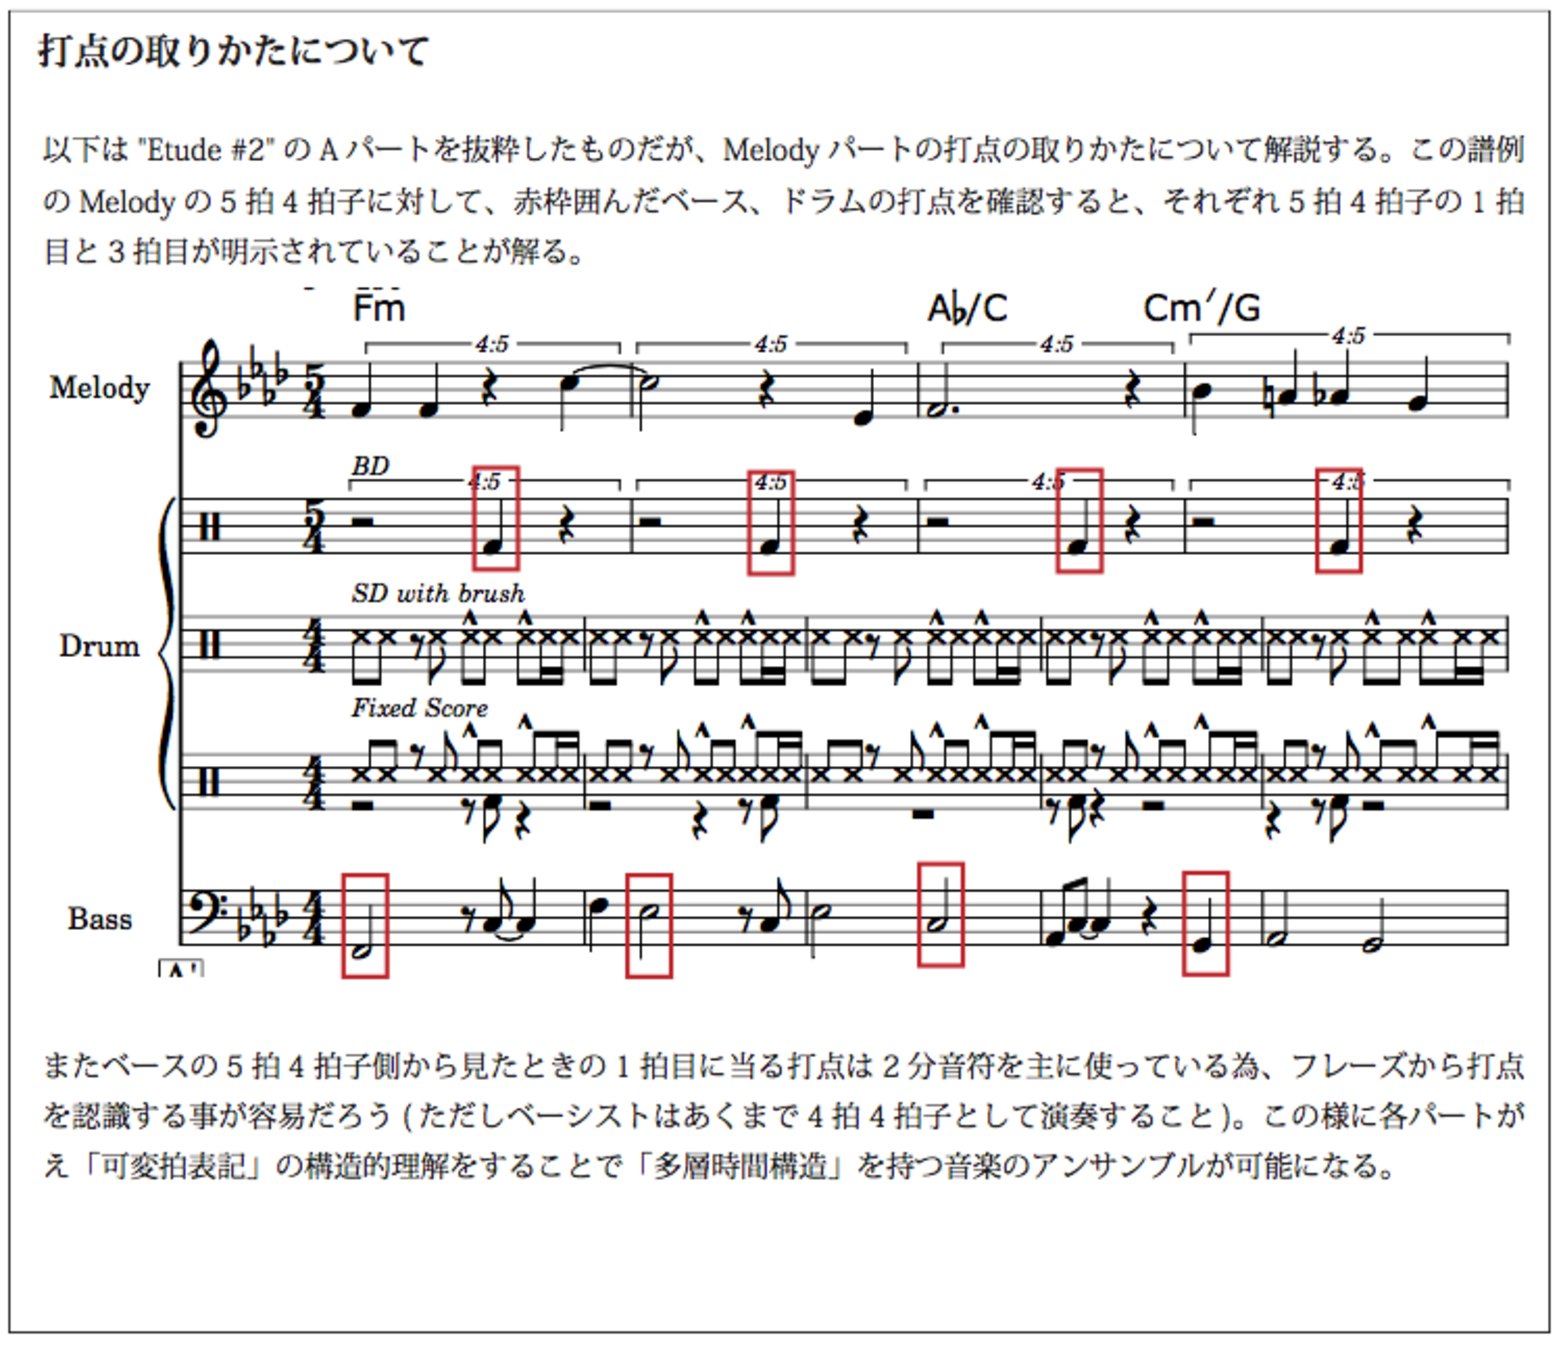
\includegraphics[
 width=\textwidth]{./PDF/figure_07.pdf}
}
\caption{''Etude \#2'' "How to take beat attack points"}
\label{fig:figure_07}
\end{figure*}

As shown in this figure, it becomes possible to generate the tempo of one's own beat from the relationships of common beats, and to read the "variable meter notation" on the time axis.

%改ページや図版を章に収めたい場合は以下のように改ページすると収まる。
\afterpage{\clearpage}
\newpage
